\chapter{Weather Balloon}
\label{chap:WB}
In this chapter we'll infer information about the ice the detectors reside in
using radio signals coming from a weather balloon flying over the stations. 
We'll go about this by first finding the difference in timing between  
channels by fitting the balloon's sinusoidal signal to the data, and
then doing a plane wave reconstruction for different indices of refraction
until we find one where the reconstructed signal gets close to the balloon.
This procedure will be explained more in depth over the following sections.

For us to find the timing we'll first make an educated guess, this can be done
using our \textit{hybrid minimizer} algorithm. There is one change that needs to
happen first to our algorithm for us to be able to simulate this: The air
observer needs to be removed as to make a ray tracing possible from
within the air into the ice and onto the detector. The modified
version of the hybrid ray tracer can be found \href{https://github.com/arthuradriaens-code/NuRadioMC.git}{here} under the branch radiopropa/BaLLooN.

Due to the way our algorithm works the time the ray took is only from when it
became a secondary\footnote{This is a problem which also seems to hold in the 
iterative ray tracer, it might get fixed in the future but as
secondaries weren't needed for most applications we deemed it fine for the
moment}, this information is insufficient as we want the full travel time.  The
propagation time from the balloon to the ice $t$ can later be added to the time
of the path in the ice by measuring the length $d$ of the drawn line from the
balloon to the beginning of the recorded path, setting the speed of radio waves
in air to the speed of light c and then just adding $t = d/c$ to the time found
from the algorithm.
\section{Plane Wave Reconstruction}
Now having modified our ray tracer, the first problem we'll consider is
plane wave reconstruction of the original position, an example path
to some of the deep sensors is given in figure \ref{fig:Example
trajectory}
\begin{figure}
	\centering
	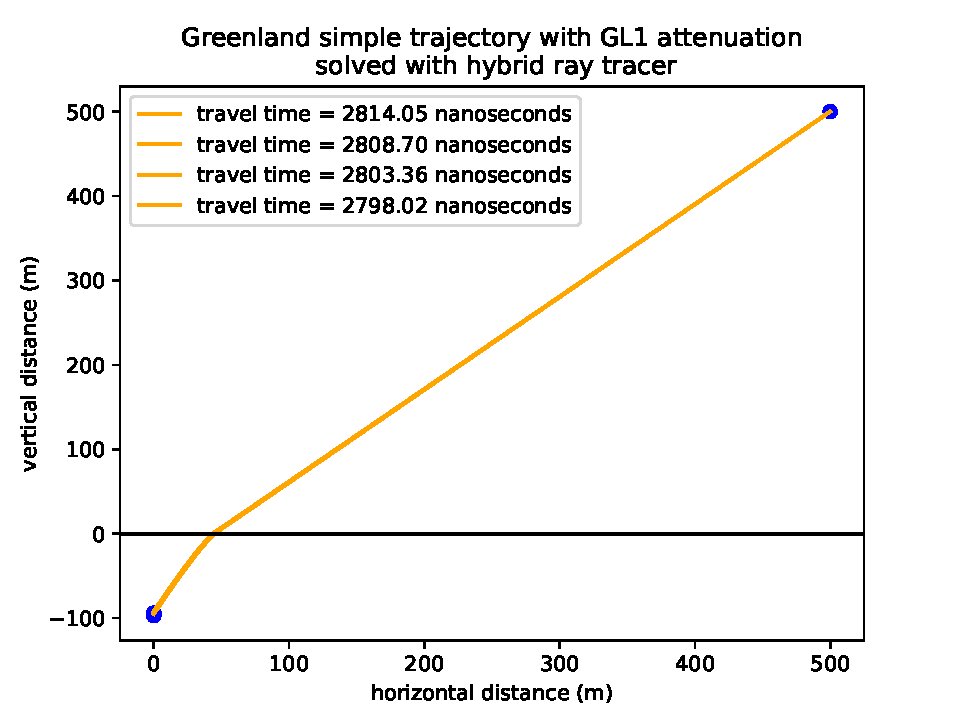
\includegraphics[width=0.7\textwidth]{weerballontraject.pdf}
	\caption{Example trajectory of rays coming from a weather balloon (blue dot top right) and going through the ice to the various detectors (blue dots bottom left)}
	\label{fig:Example trajectory}
\end{figure}
\begin{figure}
	\centering
	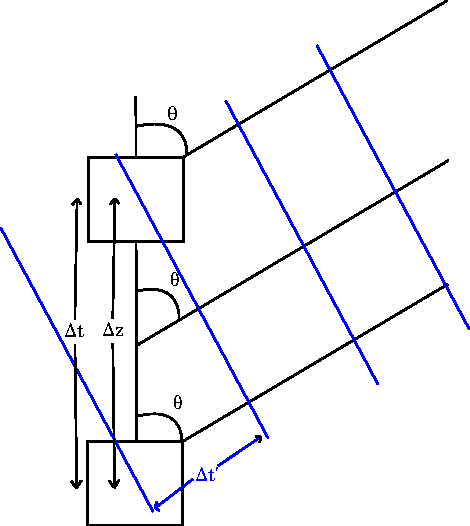
\includegraphics[width=0.7\textwidth]{planewave.pdf}
	\caption{Illustration of Plane waves}	
	\label{fig:Plane Wave}
\end{figure}
The plane wave reconstruction can easily be understood using figure
\ref{fig:Plane Wave}, the radio waves coming from the weather balloon are drawn
in blue and make a certain angle with the detectors. The top detector (top box)
detects the wave at a certain time $t_1$, the bottom detector detects it at a
time $t_2$. In our database, after decoding the signal we'd thus see that these
two detectors got a signal $\Delta t = t_1 - t_2$ seconds apart from each other.
Now ideally this is equal to the time $\Delta t'$ which is the time it took the
wave to propagate that distance which we can calculate from basic trigonometry
and dimensional analysis:
\begin{equation}
	\Delta t' = \frac{m}{(m/s)} = (s/m)*m = v^{-1} * m = v^{-1} \cos\theta \Delta z
	\label{eqn:deltataccent}
\end{equation}
With $v = c/n$ the local speed of light and n the index of refraction at the depth in between
the considered channels. 
Thus if we know the angle $\theta$, the time $\Delta t'$ and the distance between the channels $\Delta z$
we could infer the index of refraction at a certain depth as can be seen by reforming equation \ref{eqn:deltataccent}:
\begin{equation}
	n = \frac{\Delta t'}{\Delta z} \frac{c}{\cos\theta}
\end{equation}
%\begin{mintedbox}{python}
%ice = medium.greenland_simple()
%n_exact = ice.get_index_of_refraction(np.array[0,0,-95.5])
%\end{mintedbox}
In reality we don't know the angle a priori, we'll only have the recorded
timing information $\Delta t$ and the difference in channel height $\Delta z$.
So to this end we'll perform a scan by choosing some index of refraction $n_1$ and
minimizing the \textit{correlation function}:
\begin{equation}
	Correlation(\theta) := \Delta t - \Delta t' = \Delta t
	- \frac{\cos\theta \Delta z}{v}
  \label{eqn:PlaneWave}
\end{equation}
If we want to use more than 2 detectors at once however (which we'll do for the phased array), 
we'll need to specify various correlation functions.  E.g
if we have four detectors labeled 0 to 3 we'll have to construct correlation
functions between detectors 0\&1, 0\&2, 0\&3, 1\&2, 1\&3 and 2\&3 .  As all of
these correlation functions will have different sizes we'll norm them as
follows:
\begin{equation}
	Correlation_{Normed}(\theta) =
	\frac{Correlation(\theta)}{\int Correlation(\theta)\Delta
	\theta}
\end{equation}
An example simulation of these correlation functions is shown in figure \ref{fig:NormedCorrelation}. 
Notice how you can't differentiate between the correlation functions, this is only possible
because of the hybrid ray tracer having that high of a precision.
\begin{figure}
	\centering
	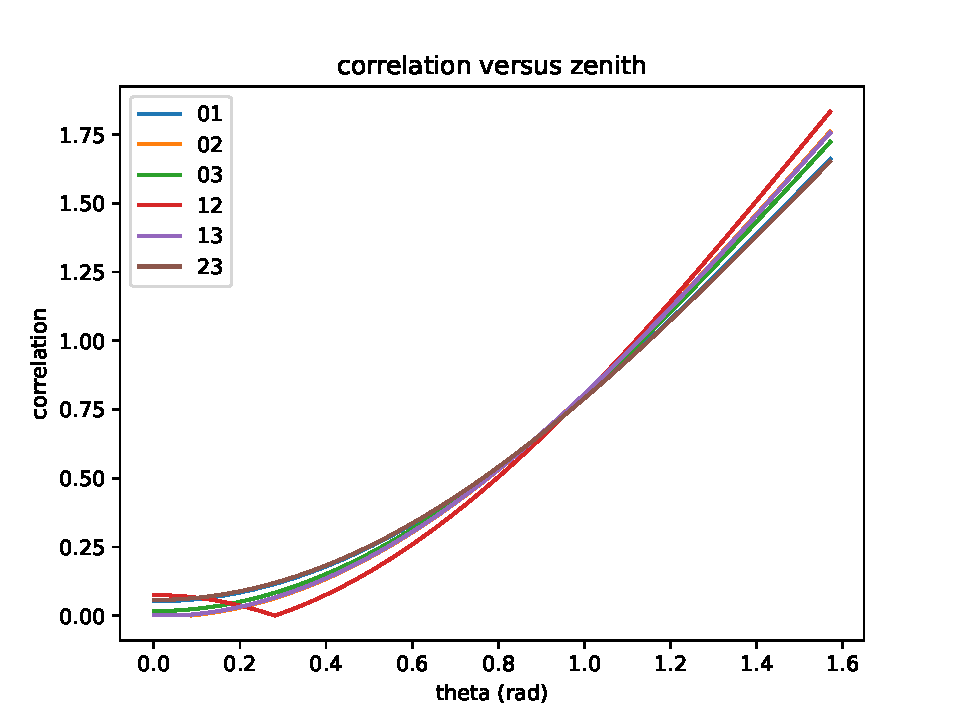
\includegraphics[width=0.8\textwidth]{NormedCorrelation.pdf}
	\caption{Example normed correlation functions}
	\label{fig:NormedCorrelation}
\end{figure}
\begin{figure}
	\centering
	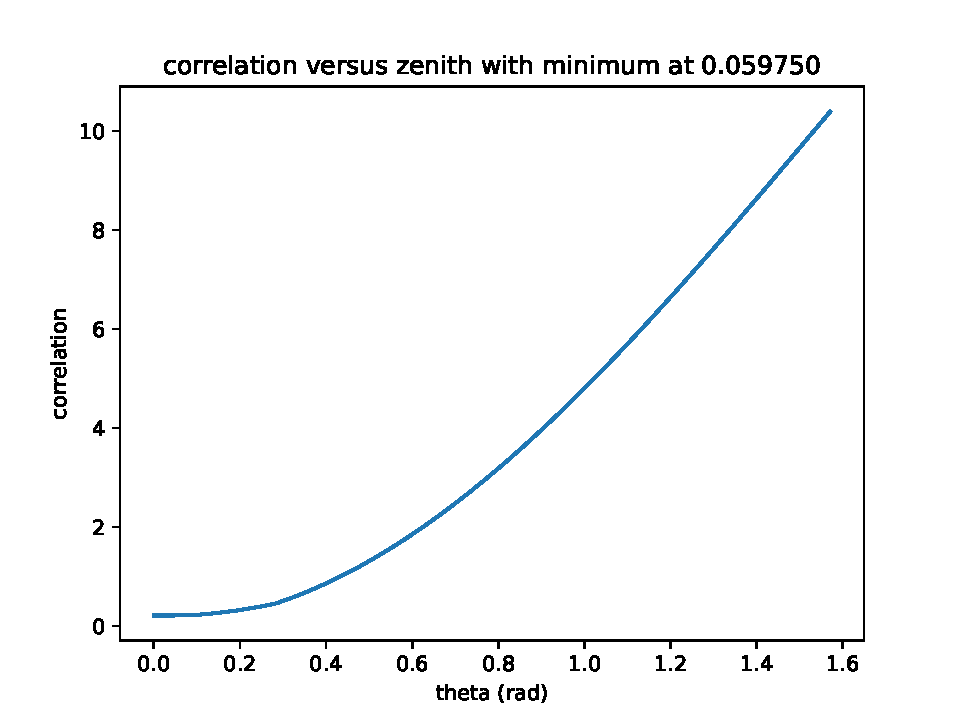
\includegraphics[width=0.8\textwidth]{SummedCorrelation.pdf}
	\caption{Example sum of the normed correlation functions}
	\label{fig:SummedCorrelation}
\end{figure}
After this we can sum them, as shown in figure \ref{fig:SummedCorrelation}, and look
at which angle it reaches it's minimum. Using this angle we can then reconstruct a ray and guess 
where the weather balloon is approximately, this is illustrated in figure 
\ref{fig:WeatherBalloonPositionReconstruction}. 
\begin{figure}
	\centering
	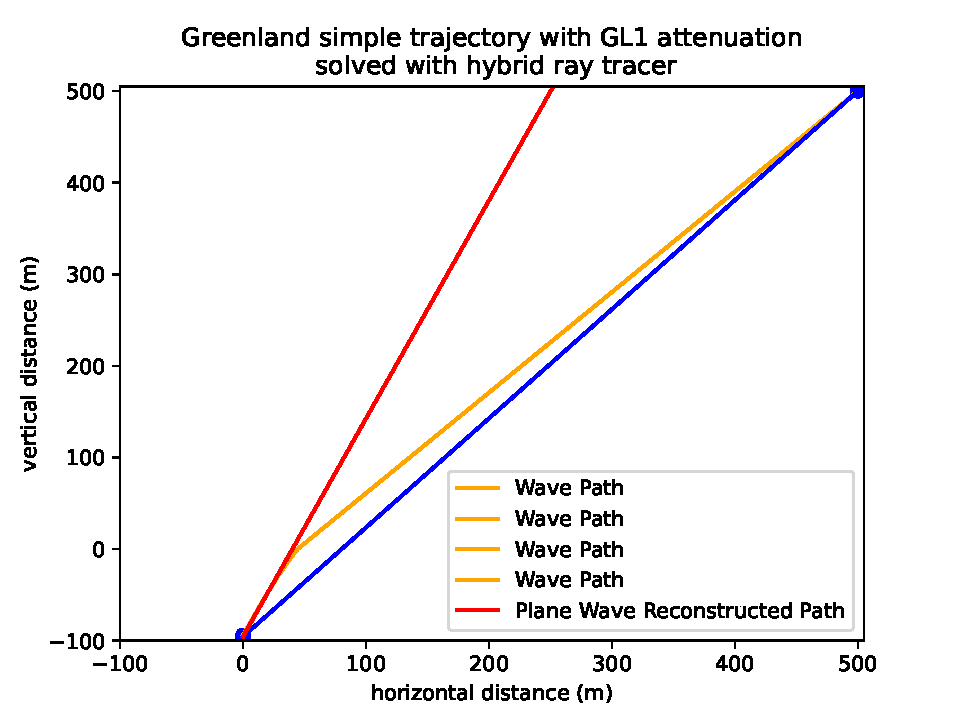
\includegraphics[width=0.7\textwidth]{WeatherBalloonPositionReconstruction.pdf}
	\caption{Example plane wave reconstruction of weather balloon position}
	\label{fig:WeatherBalloonPositionReconstruction}
\end{figure}
We can calculate the difference in distance between the weather balloon and the plane wave at the same height
and label this $d_1$, then we can choose another index of refraction $n_2$ which again corresponds to a difference
$d_2$ and so forth. At the end we take the index of refraction $n_i$ which corresponds to the minimal distance $d_i$
as the fitted index of refraction.

\section{Is the goal feasible?}
\subsection{No assumptions}
In the example reconstruction illustrated in figure
\ref{fig:WeatherBalloonPositionReconstruction} the difference in angle between
direct to balloon and plane wave reconstruction is already quite small
(0.65329617\%) but as the balloon gets closer to the detector this reduces
significantly. As previously layed out, our goal is to find the local index of refraction n by using the
plane wave reconstruction with the recorded timing and the positional data from
the weather balloon.

Now let's ask ourselves the question, within which angles should the
weather balloon fly for the data to be useful?  As was previously stated, the
further the weather balloon is away (in the x direction) the bigger the zenith
angle with the detector the less accurate the plane wave reconstruction.  So
which angles are acceptable? Note that not only angle but also height will eventually
play a role in the accuracy, the angle however gives a good starting point.
To determine this our method works as follows: 

We vary the position of the weather balloon in the x direction (keeping the
height constant at 500m), simulate the ray path to the channels 0 to 3 and then fit n
such that the difference between the balloon position and the plane wave at the same
height is as small as possible.  Then we compare the n we have fit to the
one we know from the model at that position.  We quantify the discrepancy
between these two indices of refraction using what we here define as the
\textit{correction factor}:
\begin{equation}
  \varepsilon\ (\%) = \frac{n_\text{fit} - n_{\text{exact}}}{n_{\text{exact}}} \times 100
\end{equation}
Carrying this out\footnote{The code for this can be found in
projects-mt/BaLLooN/simulations as plane\_wave.py} we get figure
\ref{fig:EpsilonIFODirect}, i.e it gets exponentially shifted towards higher n
as the balloon moves further away. If we wish our correction factor to be
within 1\%\footnote{we want this as small as possible as to not rely on the
simulation}, the angle the balloon makes with the middle of channels 0 to 3
needs to be less than 10°.
\begin{figure}
	\centering
	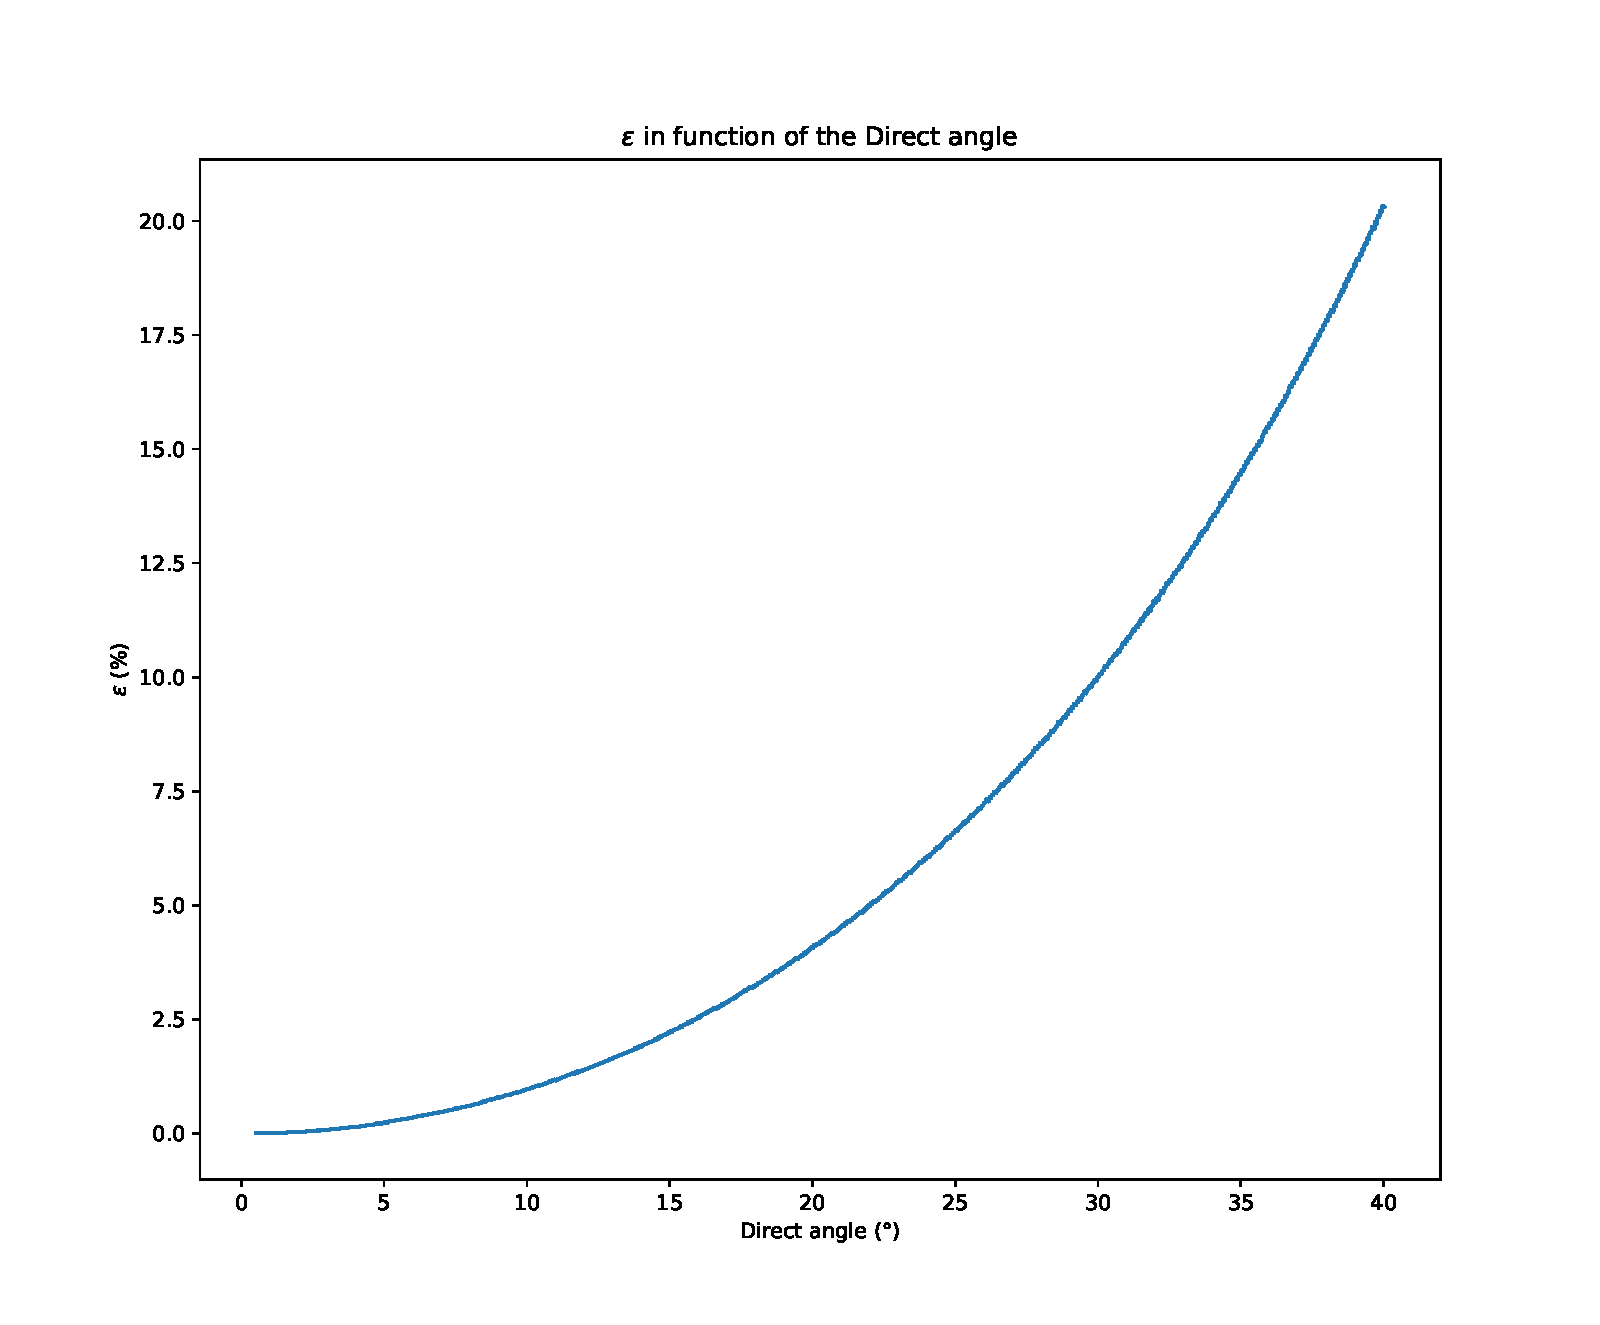
\includegraphics[width=0.7\textwidth]{EpsilonIFODirect.pdf}
	\caption{Epsilon in function of the direct angle}
	\label{fig:EpsilonIFODirect}
\end{figure}

Now what would our $<$10° policy entail? And is it even possible?  Say we take
a look at station Terianniaq (station 12) and see what our policy entails,
it is located at 72.6000868058195° N -38.4962265332872° W in the global geographic
coordinate system (longitudinal, latitude and elevation), this is quite
difficult to work with directly. For this reason we first convert the station's location to 
local ENU coordinates (east, north, up) relative to the 'DISC' which is a point in the base camp located at
72.58279265212887 latitude, -38.45581495328228 longitude and 3251.9489147560234 elevation.  

After having converted station 12's position into ENU coordinates we get
-137.67250176003688N 1727.5184983294744E, we then set our "up" to be -95.5m as
this is the approximate location of the middle of channels 0-3.  Now looking at
e.g the Balloon path recorded on the 20th of august 2022 (figure
\ref{fig:ExampleBalloonPathCrossing12}) we see that the balloon crosses paths
closely with detector 12, but how close was this encounter? To quantify this we
can take a look at every balloon positional data entry (there are $>$12000
entries) individually and compute the angle the balloon makes with the detector
by first converting the location of the balloon into ENU coordinates. Then
calculating the lateral distance ($\sqrt{(x-x')^2 + (y-y')^2}$) then the
relative vertical distance $|z - z'|$ and then from those compute the angle
($\tan(\theta) = \frac{Hor.}{Vert.}$). Doing this and recording when the balloon
gets close enough to get below the 10° mark we get the yellow part of figure
\ref{fig:ExampleBalloonPathCrossing12}. We thus see that in this
example the $<10$° policy is viable.

Now how much data do we have that way? 
We'll be looking at the data recorded over the summer of
2022, more particularly 15/06/2022 - 30/09/2022.
The positional data of the weather balloons was obtained from the
\url{ftp1.esrl.noaa.gov} website using the rno-g-sonde script of the official
RNO-G github page. After looping through every weather
balloon gpx file recorded in the summer of 2022 and seeing when it gets
within 10 degrees from any detector we get the data shown in appendix \ref{app:10Deg}, even
though this is quite a lot of data there's still another step that we could do
to broaden the amount of usable data.
\subsection{Refraction at the surface}
Up until now we have not used the property that waves refract at the surface as
we didn't want to assume anything, now say that we include refraction at the
surface for our plane wave reconstruction. This would mean that we'd follow
analogous steps as our previous analysis, i.e doing a plane wave reconstruction
from the difference in timing and trying to fit the index of refraction, only
now the plane wave abides with Snell's law at the surface, going from n=1.27 to
n=1. 

The full algorithm thus goes as follows: We first reconstruct the
plane wave launch angle $\theta_1$ by minimizing the correlation function
previously defined, we can use this angle and the height of the middle of the
concerned detectors to derive the function
\begin{equation}
	z = a_{InIce}*x + b_{InIce}
	\label{eqn:InIcePlaneWave}
\end{equation}
The outgoing zenith angle at the surface $\theta_2$ can be calculated from Snell's law:
\begin{equation}
n_1 \sin{\theta_1} = n_2 \sin{\theta_2} \implies  \theta_2 = \sin^{-1}\left(\frac{n_1}{n_2}\sin{\theta_1}\right)
\end{equation}
from this we know the slope of the wave path $a_{InAir} = \tan\left({\frac{\pi}{2} -
\theta_2}\right)$ but not the offset, but this can easily be found from equation
\ref{eqn:InIcePlaneWave} as 
\begin{equation}
	z = 0 = a_{InIce}*x_{End} + b_{InIce} \implies x_{End} = -\frac{b_{InIce}}{a_{InIce}}
\end{equation}
and 
\begin{align}
	z = 0 = a_{InAir}*x_{End} + b_{InAir} \implies b_{InAir} &= -a_{InAir}*x_{End}
	\\&= a_{InAir}* \frac{b_{InIce}}{a_{InIce}}
\end{align}
Now that we have the function describing the "path of the plane wave"\footnote{we use double
quotes as to emphasize that this is a reconstruction method and not an actual wave} in the air 
we can find out the horizontal position at the height of the balloon as
\begin{equation}
	z = z_{Balloon} = a_{InAir}*x_{f} + b_{InAir} \implies x_f = \frac{z_{Balloon} - b_{InAir}}{a_{InAir}}
\end{equation}
and iteratively loop over possible indices of refraction, minimizing $|x_{Balloon} - x_f|$.

Doing this whilst looping over possible horizontal balloon positions, we get
the result shown in figure \ref{fig:EpsilonIFODirectSnell}\footnote{The code
for this can be found in projects-mt/BaLLooN/simulations as
plane\_wave\_with\_snell.py}
\begin{figure}
	\centering
	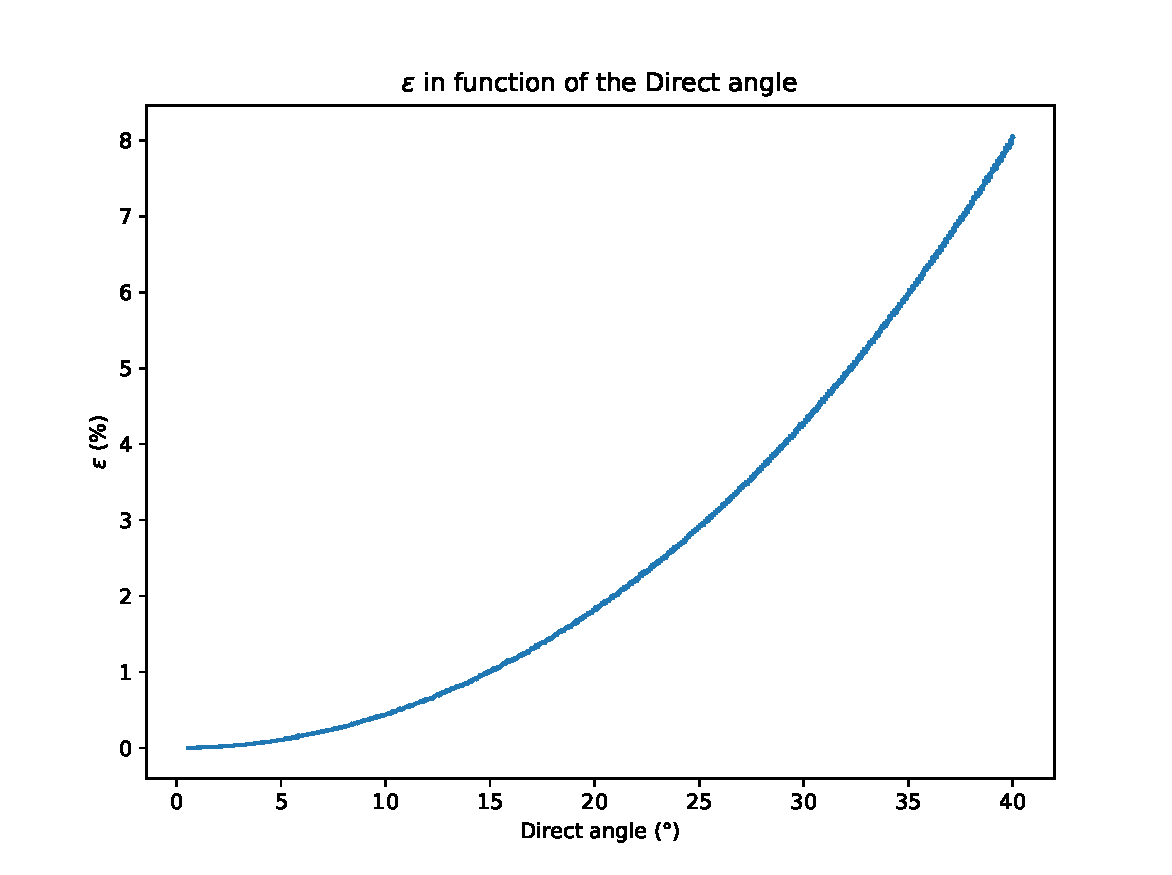
\includegraphics[width=0.7\textwidth]{EpsilonIFODirectSnell.pdf}
	\caption{epsilon IFO possible angles from channels 0-3 with refraction at the surface}
	\label{fig:EpsilonIFODirectSnell}
\end{figure}
As you can see we can now go up to 15° and still have a correction factor of less than 1\%!  The
only drawback of this method is that we need to assume the index of refraction
to be 1.27 at the surface of the ice, if this isn't the case in some places our
predictions won't be accurate.

\begin{figure}
  \centering
	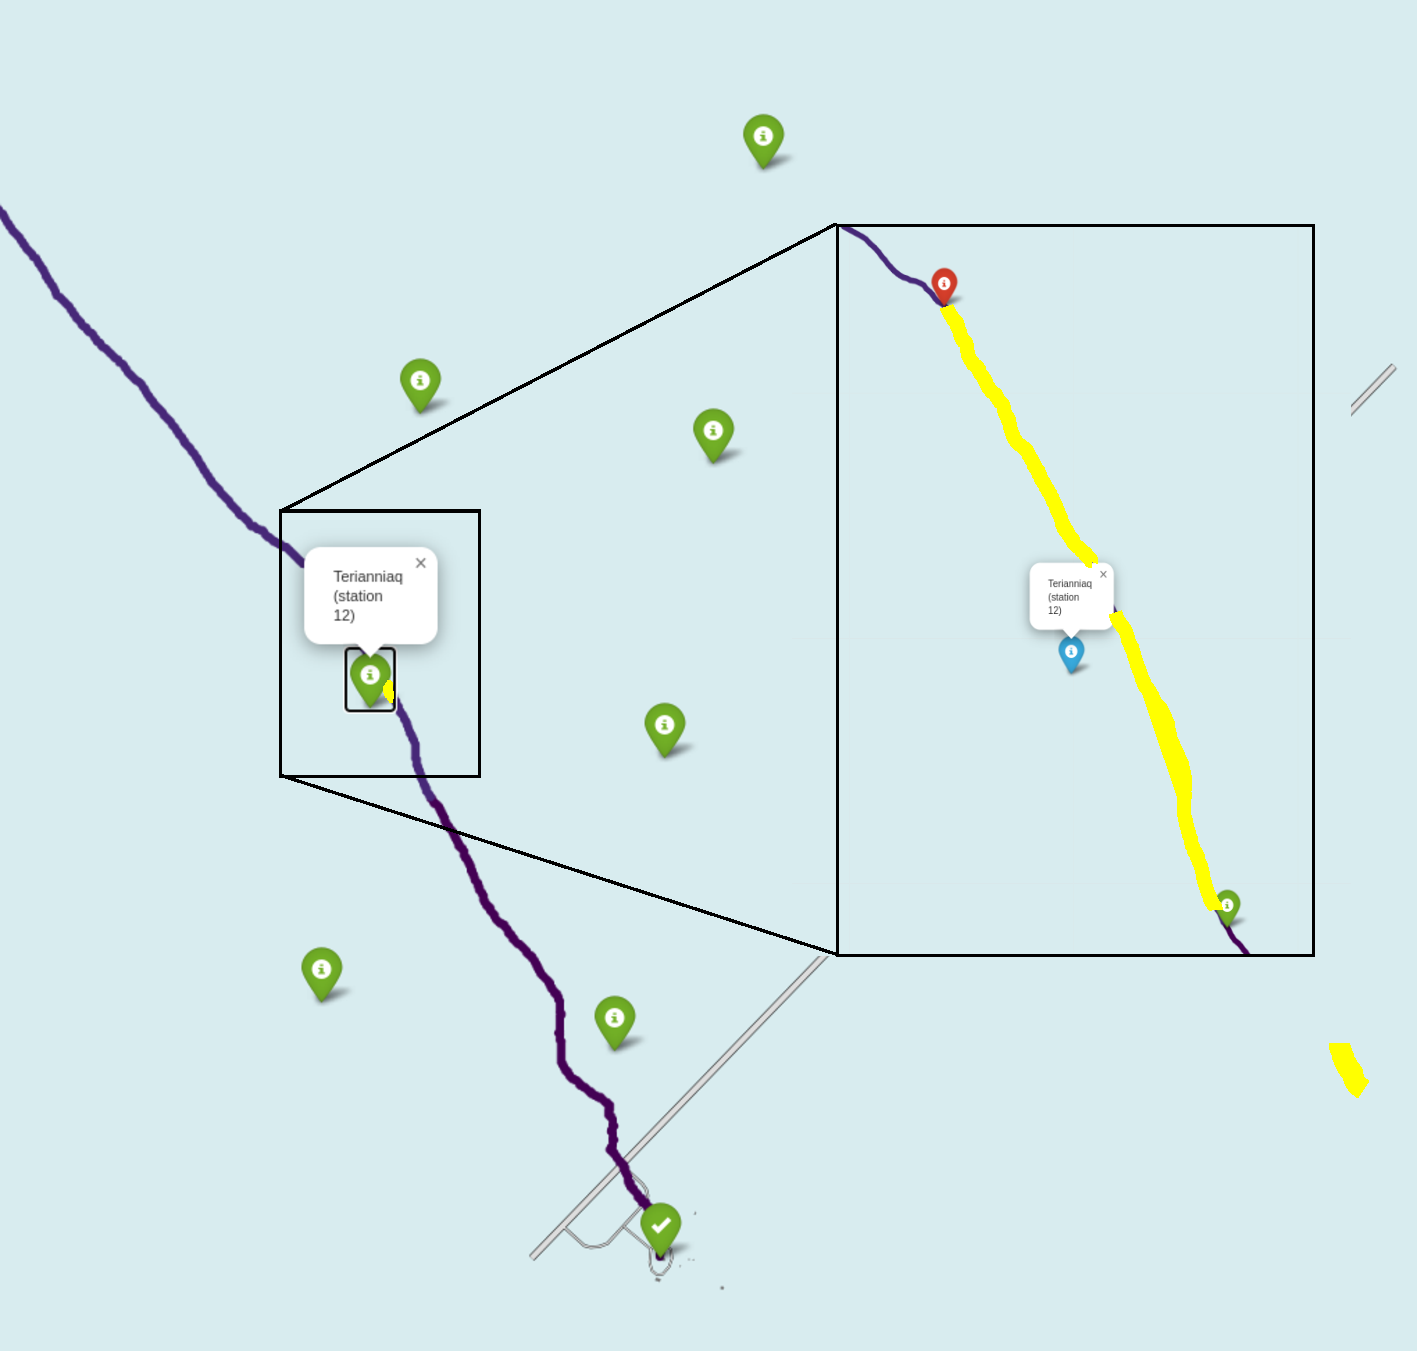
\includegraphics[width=0.7\textwidth]{BallonPathAllIllu.pdf}
  \caption{Path traced out by a weather balloon in purple released at 20/08/2022, in yellow you can see when it
  gets within 10° of detector 12.}
  \label{fig:ExampleBalloonPathCrossing12}
\end{figure}


\subsection{Influence of height on Epsilon}
In the previous sections we've assumed the height of the weather balloon to be
500m, does changing this height influence the behavior of $\epsilon$ in some
way?  The answer is, at first surprisingly, yes. As can be seen in figure
\ref{fig:EpsWithHeight} the correction factor can vary with height for the same angles.
\begin{figure}
	\centering
	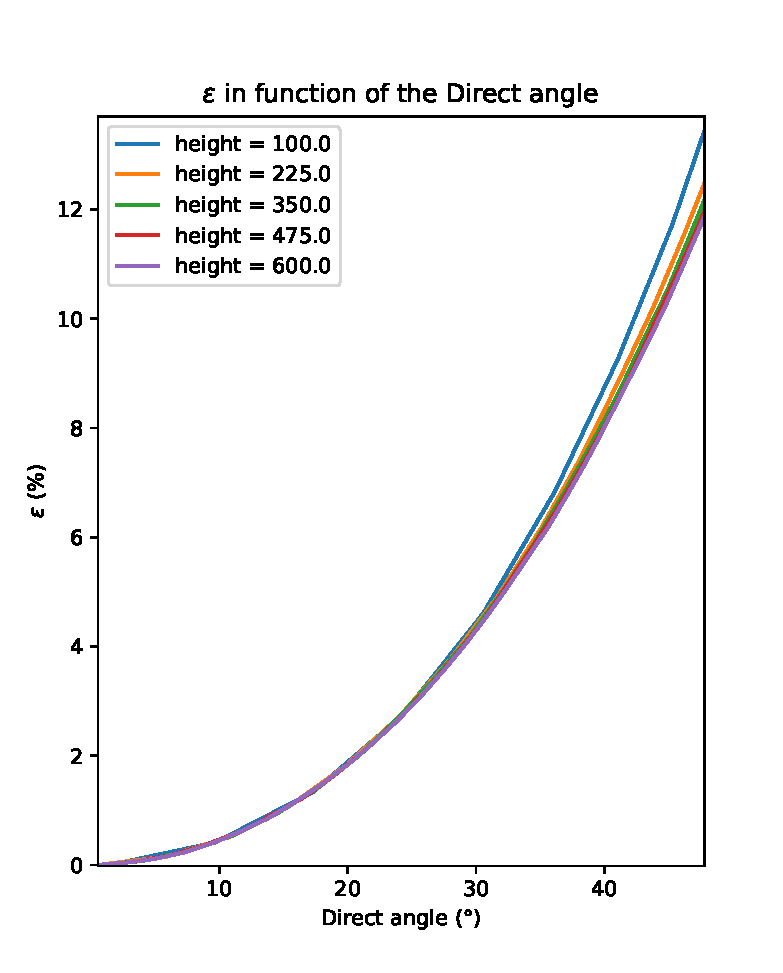
\includegraphics[height=0.4\textheight]{figures/EpsilonWithHeight.pdf}
	\caption{How varying the height influences $\epsilon$ over the same angles}
	\label{fig:EpsWithHeight}
\end{figure}
This has, as a consequence, that if we manage to get a hold on some
usable data the $\epsilon$
might still be quite large (if the height is really large).
Because of this we'll have to re-compute $\epsilon$ exactly for 
every measurement we do.
\section{Fitting the index: Phased array}
\subsection{Station 23, Run 800 Event number 1867}
Now that we know our goal to be feasible, let's analyze some data.  As we'll
start by just analyzing one event, let's take a reasonably good one for our analysis.
A close look at graph \ref{fig:EpsilonIFODirect} shows that events under 5° at
a height of 500m produce an $\epsilon$ of less than 0.22\%, implying that if we
measure n to be 1.7407 our correction factor will only be 0.0038.  A good start will
thus be finding moments when the balloon gets to within a 5\% angle, note that
the correction factor is height dependent so we'll have to calculate it afterwards.  After
looping through all the balloon positional files and only outputting the $<5$°
ones we get the time frames shown in appendix \ref{app:5Deg}.

If we search in the DESY database
\footnote{\url{https://rnog-monitor.zeuthen.desy.de/}} within the calculated
time frames for the particular detectors where the balloon gets close enough to,
and where the 403MHz signal coming from the balloon is detected in the deep channels, the events of the 7th
of September stands out; at 11:28:10,  just before the $<5$° pass by between
11:28:47 and 11:28:49, the balloon gets quite close to detector 23 and shows a
clear 403MHz signal at the phased array, as shown for the channels 0 and 3 in
figure \ref{fig:freqs03}.

Now to calculate the differences in timing for this received signal, the code
we built for this is called FitN.py and stored at the repository
\href{https://github.com/arthuradriaens-code/projects-mt.git}{projects-mt}
under BaLLooN/RealData, let's go over the full code step by step:\footnote{I advise 
the people who will continue this work to pull up the code side-by-side with this 
explanation}

\subsubsection{Spatial data}
The first part we'll need to concern ourselves with is determining the relative
positions of everything. The balloon data file and the time when the event took
place are given, from these two both the latitudinal and longitudinal position
and the elevation of the balloon at the given time are determined. We convert
these three measurements to the ENU coordinate frame (x,y,z with respect to
reference) and store it in the array \textit{BalloonPosition}. The next step is
to get the location of the detector, for this we first instantiate a detector
object 

\begin{mintedbox}{python}
det = NuRadioReco.detector.detector.Detector(json_file="RNO_season_2022.json")
\end{mintedbox}

The RNO season 2022 json file can be found on the official RNO-G github under
"analysis-tools", then we update the detector to the time of the event and get
the absolute position of our detector (station 23) via the
get\_absolute\_position module:

\begin{mintedbox}{python}
	stationlocation = det.get_absolute_position(station_id)
\end{mintedbox}

Where at the specific station this position is doesn't matter as we'll explains
shortly.  Now that we have both the position of our balloon and station in ENU
coordinates, let's simplify the calculations by setting the detector as the
origin i.e our new balloon position will be

\begin{equation}
	\textit{RelBalloon} = \textit{BalloonPosition} - \textit{StationPosition}
\end{equation}

And as we might want to plot this later, due to the cylindrical symmetry of the
ice model, we can rotate the coordinates to get rid of our y-axis. We can do
this by defining the radius:

\begin{equation}
	r := \sqrt{\textit{RelBalloon}_x^2 + \textit{RelBalloon}_y^2}
\end{equation}

And just setting this equal to $\textit{Balloon}_x$ and setting $\textit{Balloon}_y$ to
zero (equivalent to setting $\theta= 0$ in a rotation).

We don't have the position of our individual channels yet, only of the
station itself, these can however easily be obtained using the
get\_relative\_position module on our detector object. As we chose our station
to be the center of the coordinate system, these relative positions are
absolute positions of the channels in our frame of reference. Using
these it thus doesn't matter where the position of the station was defined.

\subsubsection{Signal analysis and initial guesses}
Now that we have our geometry, let's analyze the data for the channels,
the data for a particular channel is stored in a channel object. From this
object we can get the recorded voltages with the get\_trace() module, the
recorded times with the get\_times() module, the recorded frequencies with the
get\_frequencies() and the recorded spectrum corresponding to these frequencies
with get\_frequency\_spectrum() , note that the last two do a FFT on our data.
We know that the signal sent out by the weather balloon is a sine wave with a
frequency of 403MHz; as the data is measured in nanoseconds the frequency is:
\begin{equation}
	f = 403\text{MHz} = 403\times 10^{-3} \frac{1}{\text{ns}}
\end{equation}
The recorded spectrum of channels 0 and 3 is given in figure \ref{fig:freqs03}, for 
which we previously mentioned the spike at 0.403GHz.
\begin{figure}
	\begin{minipage}{0.49\textwidth}
		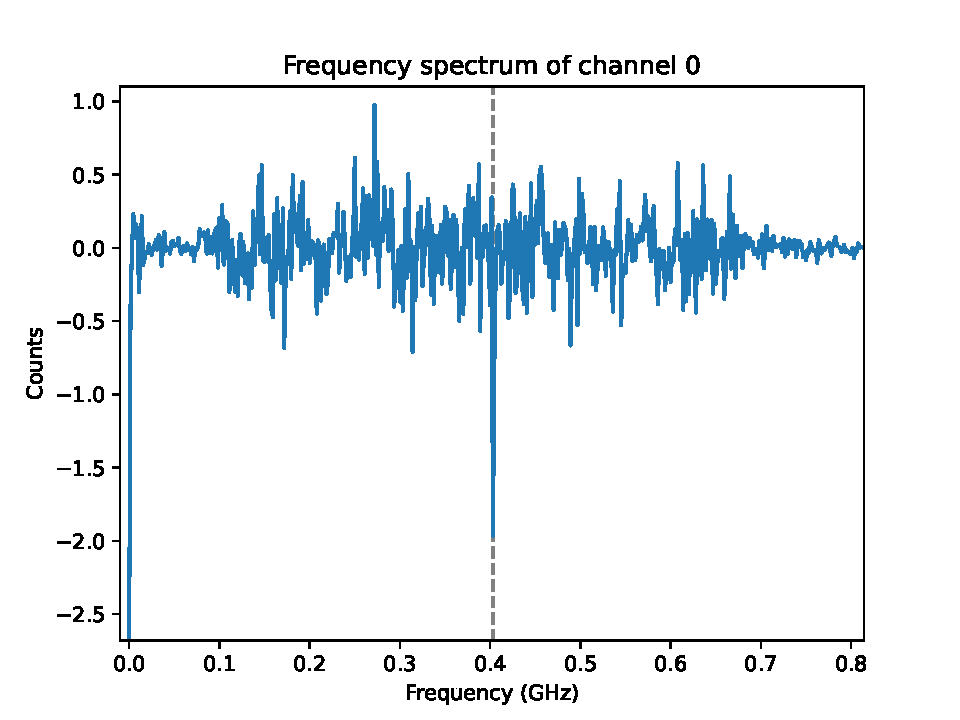
\includegraphics[width=\textwidth]{figures/23-800-0-freq.pdf}
	\end{minipage}
	\begin{minipage}{0.49\textwidth}
		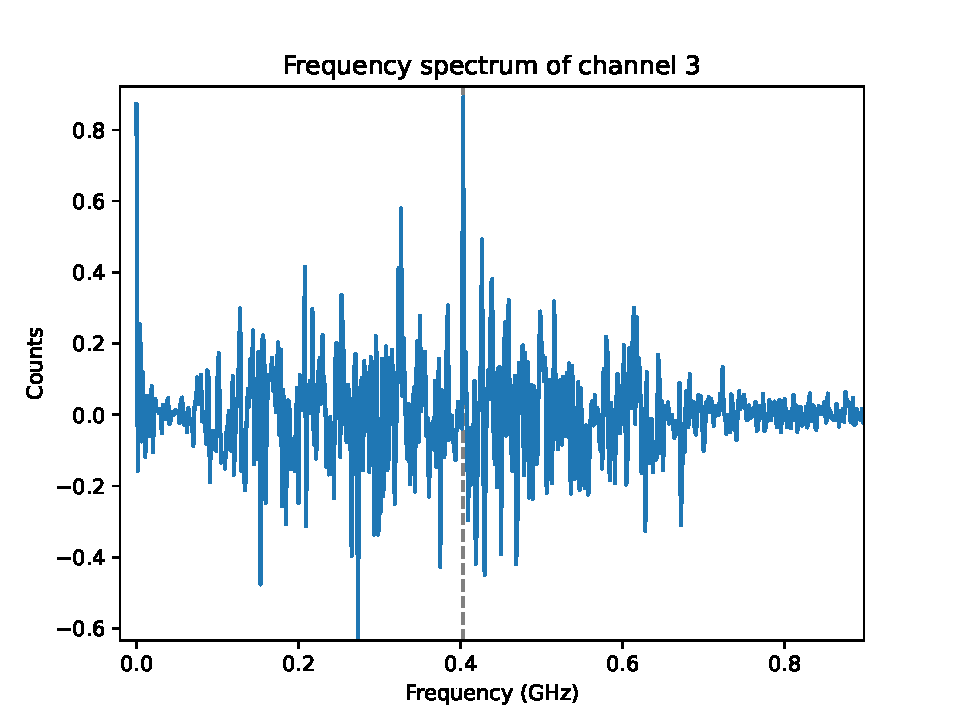
\includegraphics[width=\textwidth]{figures/23-800-3-freq.pdf}
	\end{minipage}
	\caption{recorded frequencies on detector 23 at 2022/08/29 11:18:32}
	\label{fig:freqs03}
\end{figure}
Now note that there are peaks both below 0.15GHz and above 0.6GHz,
this is all non-physical noise as the Vpol antenna's range only goes from
0.15GHz to 0.6GHz \cite{Aguilar_2021} that's why we'll first pass this signal
trough a virtual butterworth bandpass filter.

After passing the signal through the filter we'd also like to up sample the
signal as to increase the resolution, this can be done using the resample()
module and we'll up sample towards 10GHz increasing our timely accuracy from
0.3125ns to 0.1ns.  After filtering and up sampling we have some voltage
response as shown for channel 0 in figure \ref{fig:VoltageAfterFilter}, we wish
to find a sine wave coming from the weather balloon in this signal.

\begin{figure}
	\centering
	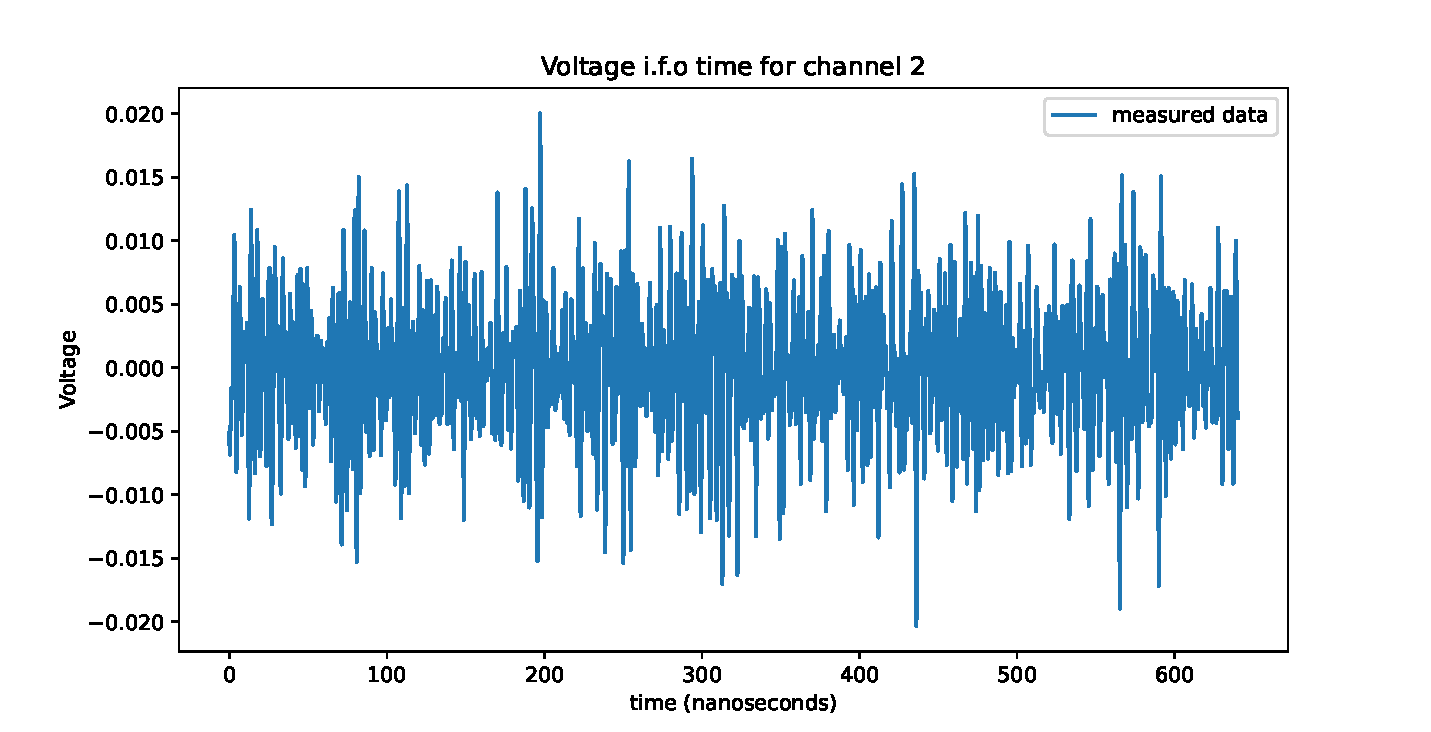
\includegraphics[width=\textwidth]{figures/VoltageAfterFilter.pdf}
	\caption{Recorded voltage i.f.o time in vpol antenna 0 after up sampling and passing through the butterworth filter}
	\label{fig:VoltageAfterFilter}
\end{figure}

To find a sine wave herein we'll use radiotools' helper module get\_normalized\_xcorr
which indirectly uses scipys signal correlation function. But before using that we'll
need a template to correlate with the data. The template we'll be choosing is
of course the sine function but it's important to notice that the channel has a
certain sampling rate, namely now after up sampling, 10GHz. 

Our template sine which we'll correlate to the data will also need to have this
sampling rate, meaning that it needs to be step wise defined with spaces of
0.1ns. Next we'll also need to give the sine a certain amplitude, as we don't
have a system for finding this yet let's for now assume an amplitude $A =
0.007$ (this shouldn't impact the correlation).  Our template thus looks like
this:
\begin{equation}
	\mathcal{S} = A\cdot\sin(\omega t) 
\end{equation}
with
\begin{equation}
	\omega = 2\pi f
\end{equation}
Herein $t$ is an array going from 0 to $3/f$ as to be able to fit 3 periods
with intervals of 0.1ns.  This template gets automatically shifted by the radiotools
correlation module with steps of 0.1ns and each time the correlation with the
data gets computed as is illustrated in figure \ref{fig:SineCorrFull}.
\begin{figure}
	\centering
	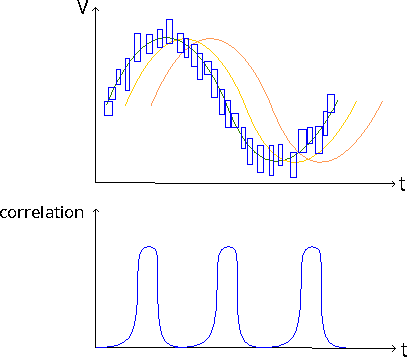
\includegraphics[width=0.8\textwidth]{figures/SineDataCorrFull.pdf}
	\caption{How correlating a sine with data leads to periodic peaks in the correlation function}
	\label{fig:SineCorrFull}
\end{figure}
In real life the data is a bit less perfect and after doing this correlation
procedure on the real data we get what's (partially) shown in figure
\ref{fig:CorrCh0}.
\begin{figure}
	\centering
	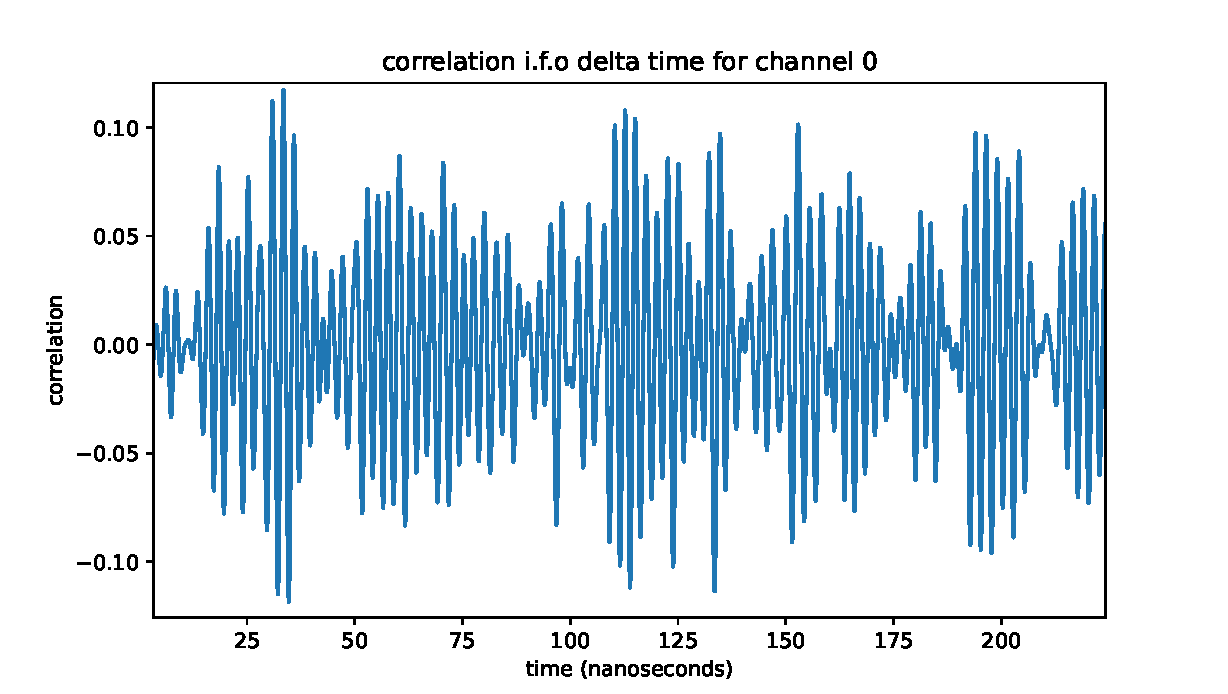
\includegraphics[width=\textwidth]{figures/CorrelationCh0.pdf}
	\caption{Zoom on the correlation i.f.o the time for channel 0}
	\label{fig:CorrCh0}
\end{figure}
Herein the peaks represent the maximal correlation, if we now do the same for
channel 3 we have two correlation functions, if we correlate these with
each other we'll get the difference in timing between the channels.  This is
easy to comprehend after taking a look at the illustration shown in figure
\ref{fig:CorrIllu}. This cross correlation is shown in figure
\ref{fig:CrossCorr}, the negative offset is caused by accounting for cable
delay. Note that multiple peak correlations are present, to thus find out which
one is the right one we'll do a simple simulation using our modified hybrid ray
tracer from which we know what the approximate time difference is and search in
this neighborhood.

\subsubsection{Fitting n and finding it's error}
Now that we have the differences in timing between the individual channels we'll loop
over the local (middle of the detectors) indices of refraction, each time doing a plane
wave reconstruction (also using Snell's law at the surface) and recording the distance
from the reconstructed wave to the balloon at the height of the balloon.
Doing this we have a list \textbf{n} and a list \textbf{differences}, if we'd select
the minimal difference in the \textbf{differences} list however we'd find an incorrect
n. We'll first need to rescale the indices using the correction factor $\epsilon$ as:
\begin{equation}
	n_{corr} = \frac{n}{1+\frac{\epsilon}{100}}
\end{equation}
If we now plot these corrected indices of refraction (which we'll from now on
just call "the fitted indices of refraction") on the x axis and on the y axis
the inverse of the differences we get figure \ref{fig:2PeakFit}. As you can
see there are 2 equally probable answers, this could be caused by the plane
wave landing left and equally distant right from the balloon. From looking at
the exponential model and the density data however we don't expect an index of
refraction as high as the second peak. We'll thus only concern ourselves with
the first peak located between 1.73 and 1.75, now we want to know what is the
exact peak value and it's error?
\begin{figure}
	\centering
	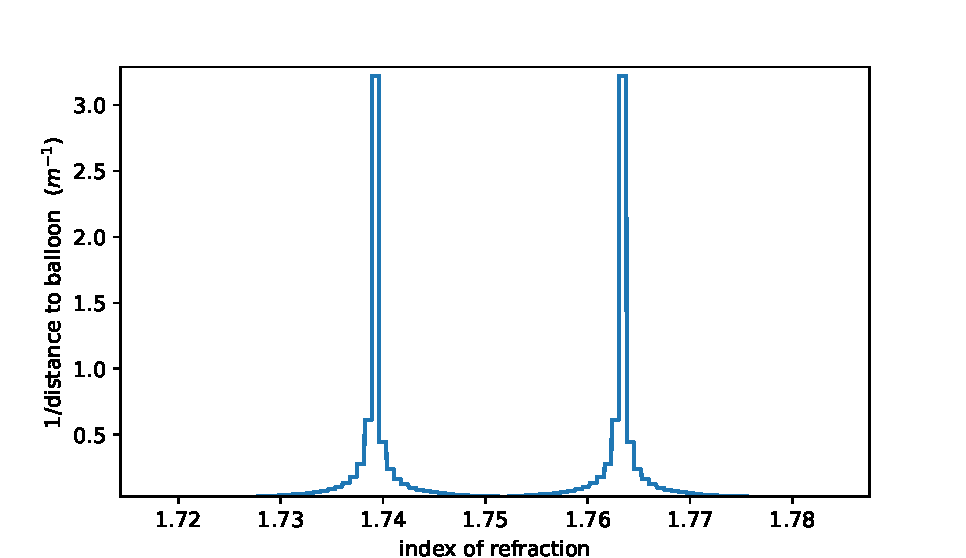
\includegraphics[width=0.9\textwidth]{TryingToFindn.pdf}
	\caption{2 possible values for n are found whilst fitting}
	\label{fig:2PeakFit}
\end{figure}

To find the peak value and it's error we'll first cut the data from
1.73 to 1.75, the value for n can be found as the middle of the
peak. To find the error on this value a first idea was to Gaussian
to this curve of the
form\cite{grabe2005measurement}
\begin{equation}
	g(x) = \frac{1}{\sigma \sqrt{2\pi}} exp\left\{-\frac{1}{2}\frac{(x-\mu)^2}{\sigma^2}\right\}
\end{equation}
the fit is shown on figure \ref{fig:GaussFit}, but as this fit obviously isn't
that great and would underestimate the error we'll need another way to find the
error.  To estimate the error we think that using integration might give a good
estimate, i.e we integrate over the full data and then again symmetrically
outwards from the middle of the peak. If the ratio of these two is 68\% then
the interval this corresponds to is the one sigma error on our fit, analogously
for 95\%. If we carry this out we get what's shown on figure
\ref{fig:PhasedArrayFit}, our final fit is thus:
\begin{figure}
	\centering
	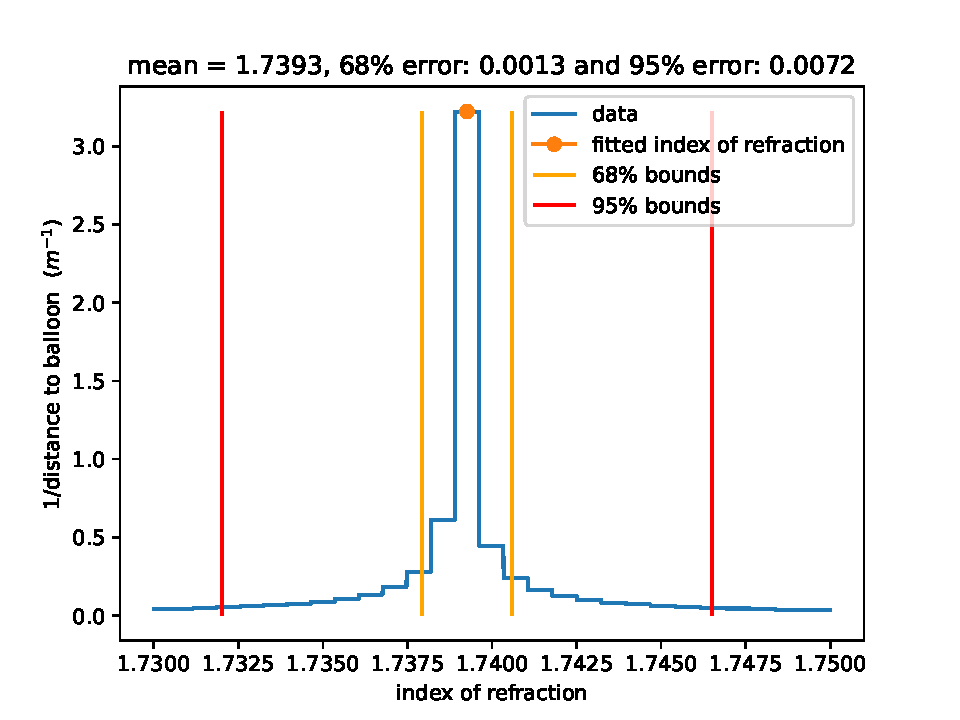
\includegraphics[width=0.7\textwidth]{PhasedArrayFit.pdf}
	\caption{Fit to the phased array data showing various confidence intervals}
	\label{fig:PhasedArrayFit}
\end{figure}
\begin{center}
\begin{tabular}{||c c c c c c c||}
 \hline
 Depth (m) & Station id & channels & Run:Event & n$_\text{exponential}$ & $\epsilon$ & n$_\text{fitted}$\\ [0.5ex]
 \hline\hline
 -93.237 & 23 & phased array & 800:1867 & 1.7383 & 4.6166\% & 1.7393 $\pm$ 0.0013 \\
 \hline
\end{tabular}
\end{center}
Here we see the index of refraction from the exponential model fall within our
fit, but note that this data isn't that reliable as the correction factor
$\epsilon$ is quite large, if we assume the correction factor to be an error on
the measured value instead of a correction we get:
\begin{center}
\begin{tabular}{||c c c c c c||}
 \hline
 Depth (m) & Station id & channels & Run:Event & n$_\text{exponential}$ & n$_\text{fitted}$\\ [0.5ex]
 \hline\hline
 -93.237 & 23 & phased array & 800:1867 & 1.7383 & 1.82 $\pm$ 0.09 \\
 \hline
\end{tabular}
\end{center}
The error on the fitted index is too large to conclude anything definitively, if we try to do 
the same reconstruction but without using snell's law at the surface a fit isn't even possible
as the index of refraction that gets found is way above 1.78 which isn't physical.
Showing just how unreliable (due to the high correction factor) this measurement is.
\begin{figure}
	\centering
	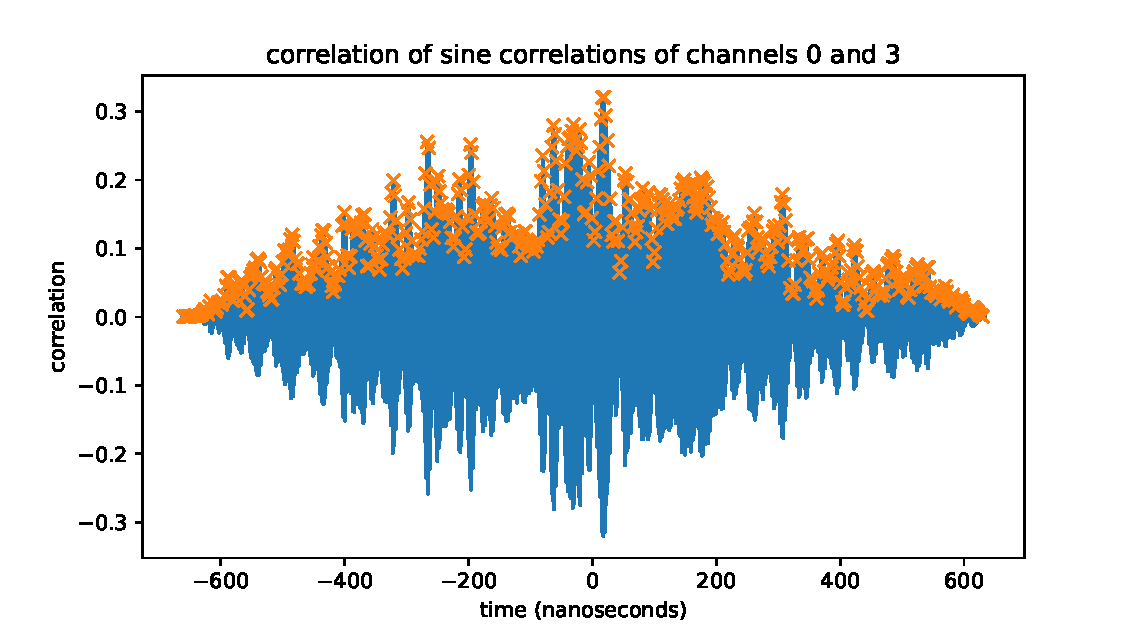
\includegraphics[width=0.9\textwidth]{figures/crosscorrelation.pdf}
	\caption{correlation of the previously, with sine, correlated data set
	of channels 0 and 3, the orange marks indicate the peaks}
	\label{fig:CrossCorr}
\end{figure}
\begin{figure}
	\centering
	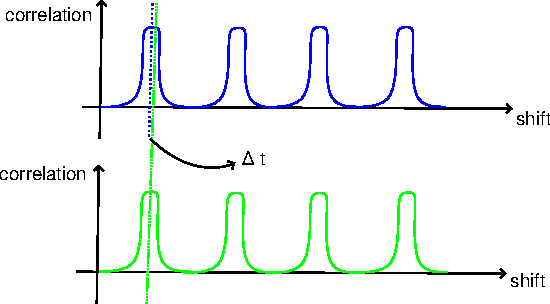
\includegraphics[width=0.9\textwidth]{figures/IlluCorr.pdf}
	\caption{Illustration of how the different correlations with sine (above
	in blue being e.g channel 0 and below in green channel 1) have a difference
in timing between the peaks which can be found from correlating the two}
	\label{fig:CorrIllu}
\end{figure}
\subsection{Station 11, Run 1034 Event number 12397}
An event triggering channels 0,2,3 is the one recorded on the 24th of july at 23:21:53,
if we reconstruct this event we get what's shown in figure \ref{fig:Event12397}.
This fit thus gives:
\begin{center}
\begin{tabular}{||c c c c c c c||}
 \hline
 Depth (m) & Station id & channels & Run:Event & n$_\text{exponential}$ & $\epsilon$ & n$_\text{fit}$\\ [0.5ex]
 \hline\hline
 -94.518 & 11 & 0\&2\&3 & 1034:12397 & 1.7397 & 0.3642\% & 1.6983 $\pm$ 0.0003 \\
 \hline
\end{tabular}
\end{center}
Which shows a very small correction factor and a clear discrepency with the
exponential model. Note that this result is less dependent on the assumptions
inherent to the ice model used in the simulation due to the small correction
factor.  
\newpage
If we take a look at the density data and convert a measurement of
roughly the same depth to the index using Shytt's equation we'd find an index
of 1.733 which also isn't in agreement with this result.
\begin{figure}
	\centering
	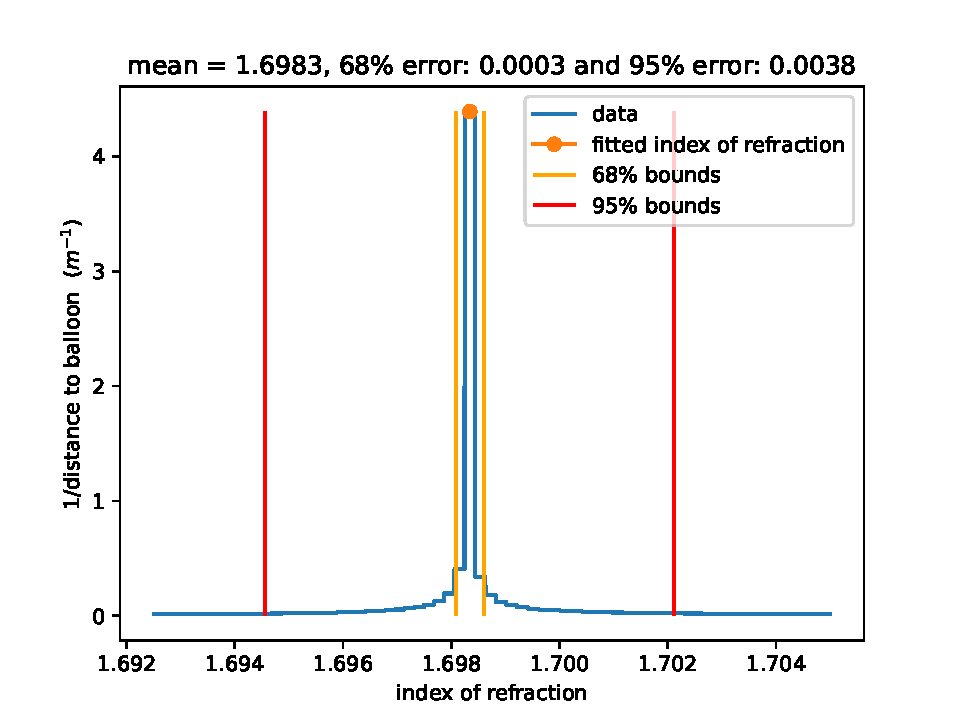
\includegraphics[width=0.7\textwidth]{figures/Event12397.pdf}
  \caption{Fit of the index on Event 12397, the peak is very narrow}
	\label{fig:Event12397}
\end{figure}
This might be caused by one of the following reasons:
\begin{itemize}
	\item Schytts law isn't fully correct
	\item The density measurements aren't correct
	\item Something went wrong in the analysis
  \item Too many assumptions
  \item Something else entirely
\end{itemize}
The density measurements do actually show quite a lot of spread for nearly
the same values so there might be a problem there (there are also not that many
recorded measurements and no reported uncertainties).  

As for the Schytt's equation, whether it is a valid approximation or not will be
decided when enough reliable data is available.  

Only careful scruteny of the algorithm and code  used throughout this work will tell
if something went wrong with the analysis or something else enterily (e.g the importance of birefringence).

To do away with some assumptions made, we also redid the fit using only the
plane wave method, not making use of snell's law at the surface. Doing this the
only assumptions that gets made is that the signal ends up approximately at the
same time as in the simulation ($\pm$ half the period of the signal) and that
the index gets corrected the same way but this gave the same value.

Let's lastly consider the case where we see the correction factor as an error on the measurement, this would give
\begin{center}
\begin{tabular}{||c c c c c c||}
 \hline
 Depth (m) & Station id & channels & Run:Event & n$_\text{exponential}$ & n$_\text{fit}$\\ [0.5ex]
 \hline\hline
 -94.518 & 11 & 0\&2\&3 & 1034:12397 & 1.7397 & 1.7045 $\pm$ 0.006 \\
 \hline
\end{tabular}
\end{center}
This value is the most trustworthy we have as it doesn't assume \textbf{anything} about the
ice, note how it \textbf{still disagrees with the exponential model}, how much it disagrees
is clearly shown in figure \ref{fig:IndexVSDepth.pdf}.
\section{Channels 5,6 and 7}
A very interesting depth is in between channels 5 and 7 as, looking at the
difference between the index computed from the density and the single
exponential model as shown in figure \ref{fig:IndexVSDepth.pdf} this is where
the largest deviations between both is observed. We'll take a look at this
depth with channels 5,6 and 7 but note  that these will be way less reliable
(difficult to quantify how unreliable) than the phased array as the channels
are spaced too far apart. \textbf{This is thus only performed as a test and
the data shouldn't be taken seriously}.

The event we'll be using is recorded in detector 21 at the 26th of July
11:18:41 and falls within the $<5$° mark, doing analogous analyses as in the
previous section we get figures \ref{fig:Ch5And6}-\ref{fig:Ch5And7} which can
be summarized in a table as shown below:
\begin{center}
\begin{tabular}{||c c c c c c c||}
 \hline
 Depth (m) & Station id & channels & Run:Event & n$_\text{exponential}$ & $\epsilon$ & n$_\text{fit}$\\ [0.5ex]
 \hline\hline
 -48.155 & 21 & 6\&7 & 1441:117 & 1.6400 & -0.02\% & 1.6310 $\pm$ 0.001 \\
 -58.38 & 21 & 5\&7 & 1441:117 & 1.6736 & -0.23\% & 1.6688 $\pm$ 0.0006 \\
 -68.2 & 21 & 5\&6 & 1441:117 & 1.6983 & 0.02\% & 1.6916 $\pm$ 0.0003 \\
 \hline
\end{tabular}
\end{center}
Note that all of the indices that are found have a value below the
exponential model's.
\begin{figure}
	\centering
	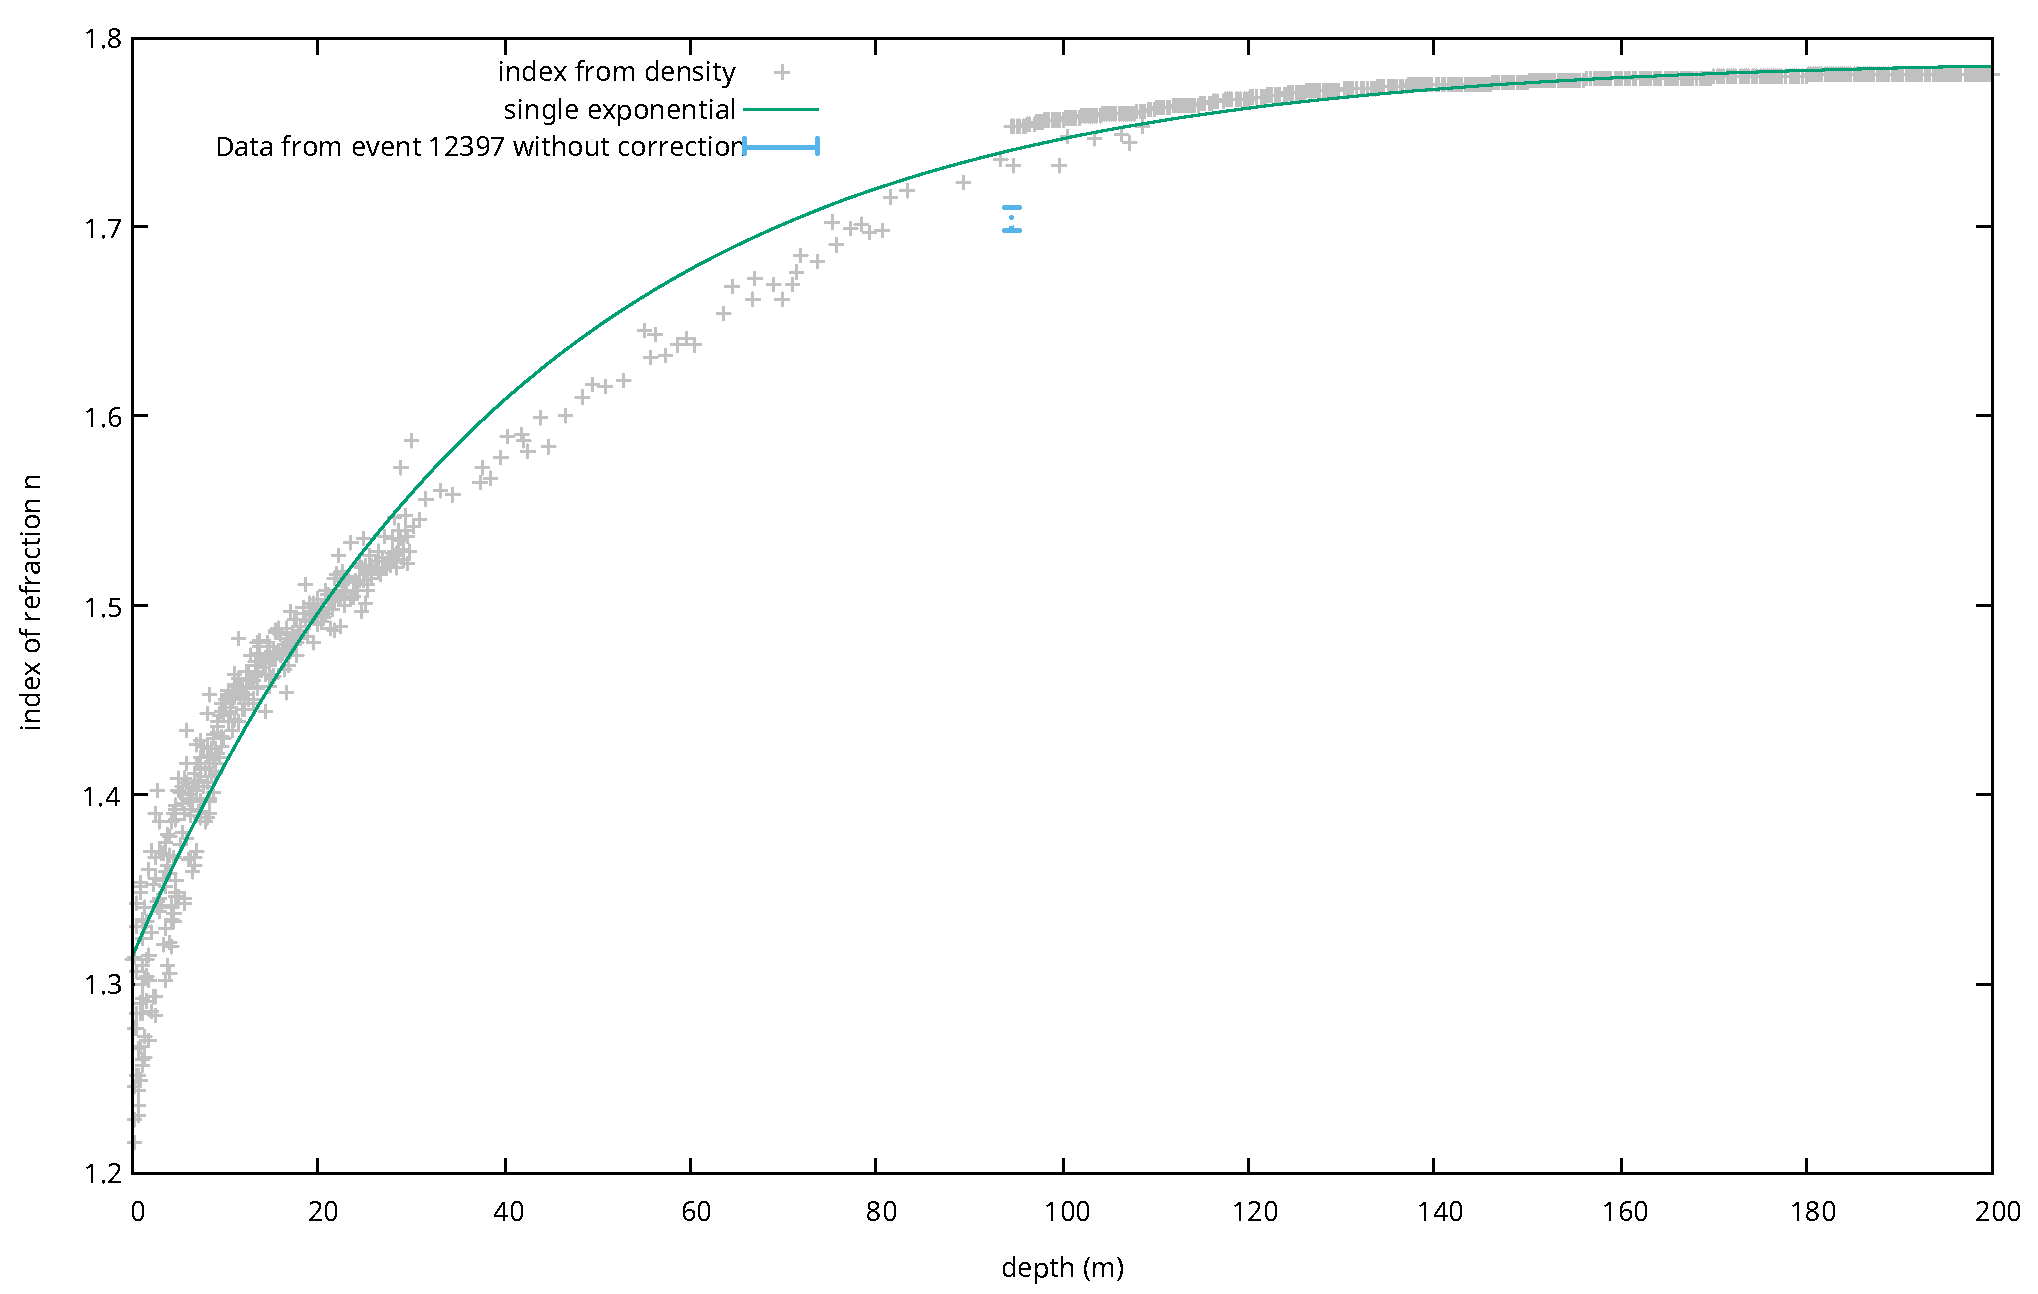
\includegraphics[width=0.8\textwidth]{figures/Event12397NoCorr.pdf}
  \caption{Event 12397 shows itself as a clear outlier hinting at the need to investigate the index-depth relation further}
	\label{fig:IndexVSDepth.pdf}
\end{figure}
\section{Guide for further analysis}
Here I'll give a quick guide on how to continue this work, as a phased array
measurement with small error hasn't been found yet.  First off you'll need to
install the NuRadioMC fork from my github located
\href{https://github.com/arthuradriaens-code/NuRadioMC.git}{here} and checkout
the branch radiopropa/BaLLooN. Then go to
\url{https://rnog-monitor.zeuthen.desy.de/} and search for events mentioned in
appendix \ref{app:5Deg} (within those time frames), looking at the frequency
spectrum of the phased array to see if the 0.403GHz signal gets detected. If
such an event gets found write the run and event number down and also the exact
date and time.

Now download this run file, the exact procedure is explained on the rno-g
internal wiki under "analysis" but after you have installed everything my
"getrnorun.sh" script located
\href{https://github.com/arthuradriaens-code/Scripts.git}{here} might come in
handy.

Now download all the balloon positional files (.gpx files) with the rno-g-sonde
script located \href{https://github.com/RNO-G/rno-g-sonde.git}{here} and in
this find the balloon file relevant for the event time, e.g a file named
"SMT\_20230315\_111501.gpx" was launched the 15th of march in 2023 at 11:15:01. 

Now the preparations are done, download the program used for fitting called
"FitN.py" located
\href{https://github.com/arthuradriaens-code/projects-mt.git}{here} under
BaLLooN. If you take a look at it's source code the first few variables
(station\_id, event\_id, gpx\_file,...) are what need to be changed to the
previously found values. Run this with n\_cut=None and then look at a good cut
for the index of refraction (over which range you want to do the error
analysis, examples are shown in appendix \ref{app:EF}) and rerun the program.
